\itemhead{习题1.1 · 第13题（教材p.13）}{XJ-B1-C01-HW-P013-Y0922}
\label{XJ-B1-C01-HW-P013-Y0922}
{\footnotesize 湘教版教材p.13 / PDF第20页 / 习题1.1 / 第13题}
\field{原题}{设 $U$ 是全集，$A$，$B$ 是 $U$ 的两个非空子集，$A\cap B\ne\varnothing$，用 Venn 图表示：
\subq{1}$A\cap(\complement_U B)$；
\subq{2}$B\cap(\complement_U A)$；
\subq{3}$(\complement_U A)\cap(\complement_U B)$；
\subq{4}$(\complement_U A)\cup(\complement_U B)$。}
\field{参考答案}{Venn图依次涂：只属于 $A$ 的部分；只属于 $B$ 的部分；两集合以外的部分；除 $A\cap B$ 外全集内全部部分。对应 $A\setminus B,B\setminus A,U\setminus(A\cup B),U\setminus(A\cap B)$。}
\begin{center}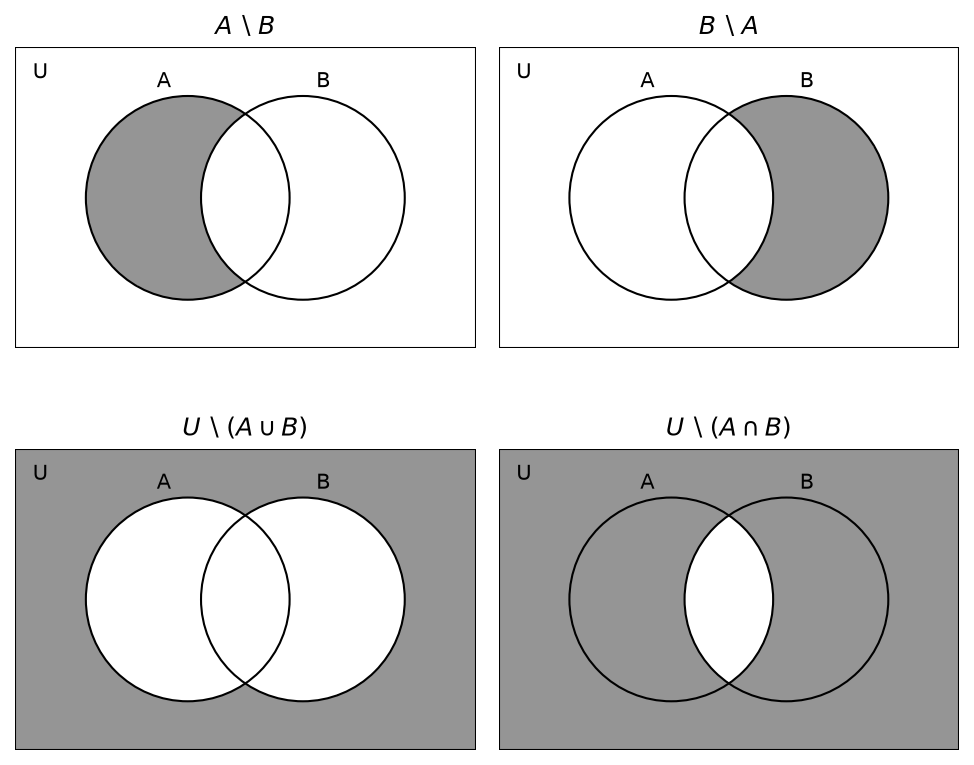
\includegraphics[width=.84\linewidth,height=.38\textheight,keepaspectratio]{figures/C01-HW013-13.png}\end{center}
{\small \field{关联知识}{S04 交集、并集及解集的联系（教材帮p.19、20 / PDF28、29）；S05 全集、补集与德摩根律（教材帮p.21 / PDF30）}
\field{方法与易错点}{先各自化简集合或解出约束，再在数轴上合并；有序数对交集通过联立方程求得。 易错：并集重复写元素；连接处一个闭端点也误删；把交集当并集。}
\field{答案依据}{答案册相关题组：PDF第4、5页（册内页3、4）；按当前题库原题逐项重算，不按旧版题号机械对套。}}
